\subsection{Background}
Our focus will be applying the Finite Volume (FV) scheme to solve linear and non-linear hyperbolic PDEs in first order form.
We express these PDEs mathematically with the equation
% See exahype template
\begin{equation}\label{eq:non-lin-pde}
    \frac{\partial \mathbf{Q}}{\partial t}(x,t) + \nabla \cdot \mathbf{F}(\mathbf{Q}) + \mathbf{B}(\mathbf{Q}) \cdot \nabla \mathbf{Q}(x,t) = \mathbf{S}(\mathbf{Q})
\end{equation}
where $\mathbf{Q}(x,t)\subset \mathbb{R}^q$ is a time and space dependent state vector for any $x$ in our spatial domain $\Omega\subset \mathbb{R}^{d \in \{2,3\}}$ and $t>0$.
The number of conserved state variables, $q$, can vary from $5$ in the 3D Euler Equations, $58$ in the Einstien Relativity equations (CCZ4) \cite{CCZ4}.
$\mathbf{F}$ is the conserved flux vector, $\mathbf{B}$ the (system) matrix composing the non-conservative fluxes and $\mathbf{S}(\mathbf{Q})$ the source term.
The $\mathbf{B}(\mathbf{Q}) \cdot \nabla \mathbf{Q}(x,t)$ term is often called the NCP (non-conservative product).


We will derive the FV scheme for  (\ref{eq:non-lin-pde}) in the case that $B(Q)=S(Q)=0$
\begin{equation*}
    \frac{\partial \mathbf{Q}}{\partial t} + \nabla\cdot \mathbf{F}(\mathbf{Q}) = 0.
\end{equation*}
FV begins by dividing the spacial domain into finite volumes, known as cells.
For a cell, $i$, we take an integral over its volume $v_i$
\begin{equation*}
    \int_{v_i}\frac{\partial \mathbf{Q}}{\partial t}\,dv + \int_{v_i}\nabla\cdot \mathbf{F}(\mathbf{Q})\,dv = 0.
\end{equation*}
Then we integrate the first term to give the average state $\bar{\mathbf{Q}_i}$ over the cell, and apply divergence theorem to the second term
\begin{equation}\label{eq:fv-almost-done}
    v_i\frac{\partial \bar{\mathbf{Q}_i}}{\partial t} + \oint_{S_i}\mathbf{F}(\mathbf{Q})\cdot \mathbf{n} \, dS = 0
\end{equation}
where $S_i$ is the surface of cell $i$ and $\mathbf{n}$ is the outward facing normal vector.
Rearranging (\ref{eq:fv-almost-done}) for the time derivative we find
\begin{equation}\label{eq:fv-done}
   \frac{\partial \bar{\mathbf{Q}_i}}{\partial t} = -\frac{1}{v_i} \oint_{S_i}\mathbf{F}(\mathbf{Q})\cdot \mathbf{n} \, dS.
\end{equation}

If we select an simple geometry for our cell, squares/cubes are used in ExaHyPE, then calculating the 2D surface integral is simply a sum across the 4 faces of a square (or in 3D, the 6 faces of a cube).
Asserting $S_i$ is a finite set of faces allows us to simply the surface integral
\begin{equation}\label{eq:fv-simple}
   \frac{\partial \bar{\mathbf{Q}_i}}{\partial t} = -\frac{1}{v_i} \sum_{S_i}\mathbf{F}(\mathbf{Q})\cdot \mathbf{n}.
\end{equation}
This provides a method to calculate the time derivative of $Q$, which can be used in a time stepping scheme such as explicit Euler to progress $Q$.


\subsection{ExaHyPE}
\newcommand{\proc}[1]{\textit{#1}}
Algorithmically a FV cell is an array of \texttt{double}.
In ExaHyPE cells are grouped up into patches, commonly $3\times 3$ cells in 2D or $3\times 3 \times 3$ cells in 3D, and these patches are store as an AoS (Array of Structures).
The Peano framework within ExaHyPE is responsible for distributing these patches across processing cores and nodes, where they are updated using (\ref{eq:fv-simple}) and an explicit euler time stepping scheme, by a single core.
We will refer to this update process as \proc{Patch Update}.
As an aside, In (\ref{eq:fv-simple}) we set $B(Q)=S(Q)=0$ for simplicity, however in the case $B(Q), S(Q)\neq 0$ the update process is broadly similar to (\ref{eq:fv-simple}), the main feature of which being a sum across the faces of a cell.

An issue encountered in (\ref{eq:fv-simple}) is: what is the value of $Q$ at a face?
Take a the face between cells $\alpha$ and $\beta$.
We know the average state across $\alpha$ which we call $Q_\alpha$, and likewise for $\beta$ with average state $Q_\beta$.
However the face, $f$, lies on the boundary of $\alpha$ and $\beta$ the state of which is a discontinuity between $Q_\alpha$ and $Q_\beta$ so what should $Q_f$ be?
This is know as the Riemann problems.
Simple solutions exist, such as taking an average $Q_f = \frac{Q_\alpha + Q_\beta}{2}$, and the best choice of scheme is problem specific.
By default, ExaHyPE uses the Rusanov scheme \cite{rusanov} as a general purpose solution to the Riemann problem, however user have the option to provide their own scheme.
Once a value of $Q_f$ has been decided upon then $F(Q_f)\cdot \mathbf{n}$ (and additionally NCP terms if applicable) can be calculated.
We call this process the \proc{Numerical Ingredient}, and we can trace it back to the evaluation of $F(Q)\cdot\mathbf{n}$ in (\ref{eq:fv-simple}).

Adding further complexity to \proc{Numerical Ingredient}, it is not always the case that we want to model the face between $\alpha$ and $\beta$ as a shared face.
Sometimes we treat $f$ as two faces $f_\alpha, f_\beta$, which means we cannot assume that evaluating the \proc{Numerical Ingredient} while updating $\alpha$ will be the same as when updating $\beta$.
The Rusanov scheme used by default in ExaHyPE doesn't experience this complication, treating the face as a shared face. 
Thus, this is a good example of ExaHyPE supporting functionality which is not required by default, but may be required for certain problems.
And, this support adds additional barriers to optimisation.

Referring back to (\ref{eq:fv-simple}), a user must provide code to calculate $F(Q)\cdot\mathbf{n}$, which we will call one of the \proc{Problem Descriptions}.
If their equation has a non-zero source term and NCP term a user will also need to provide code to calculate these quantities.
Additionally Rusanov and mesh/timestep refinement requires the max-eigenvalues of a cell, so this must also be provided by the user.
Finally a user will need to provide code that describes the boundary conditions of the problem.
This is all the code a user needs to provide.

These 3 process are split into 3 functions in ExaHyPE, a summary of the number of inputs and outputs of these functions can be found in Table \ref{tab:patch_update}.



% Can we make exahype better
% while not making it worse

% we will focus on patch update
An ExaHyPE project is a majority of engine code, and a small amount of user code which is used to describe the PDE.
The interface between the engine and user code is built on the patten of passing function pointers of user functions to engine code.
Here is an example:
\begin{lstlisting}[language=c]
void engine_function(std::function<...> user_function){
    // ... Do something
    val = user_function();
    // ... Use the value of the user function 
}

void engine_core(){
    auto user_func = project::user_land::foo;
    engine_function(user_func);
}
\end{lstlisting}

This patten is good design practice, as it completely decouples engine functions from user functions, apart from at a single crossover point.
Thereby allowing the engine to be developed in isolation from user codes, and allowing the engine to support any user codes that respect the required function signatures.
However, this patten, and the total disconnect between user and engine code it allows, is not without its disadvantages, as we will discuss.

Our focus will be on the \proc{Patch Update} process.
This process is heavily reliant on user code, and as such dominates the runtime of user code.
Furthermore, for arithmetic intense PDEs, this process dominates the entire running time of an ExaHyPE program.
We will begin by explaining the \proc{Patch Update} process.
Then proceed to highlight inefficiencies within this process. 

The smallest unit of space in a FV scheme is a cell.
Algorithmically a cell is an array of \lstinline{double} that store the state of that cell.
As mentioned previously the size of the state vector can vary from $4$ values to over $40$.
Cells are then grouped up into a patch.
Within ExaHyPE, patch data is stored in a AoS (Array of Structures) form.
Patch sizes are typically 3x3 cells in 2D or 3x3x3 cells in 3D.
The size of patches can be adjusted by a user, say to 5x5, however a patch size is a constant throughout the runtime of the program.
Within ExaHyPE, the Peano Framework \cite{PeanoFramework} is responsible for splicing the spacial domain into patches, and distributing patches across compute nodes and compute threads.
As such, we are concerned with the single threaded process of \proc{Patch Update}.
\proc{Patch Update} is used to evolve the values of cells in a patch by a given timestep.
This is done by applying source terms to the cells, then calculating flux and non-conservative products (NCP) for every face of a cell and applying it to the cells state.
As a technical detail, to evaluate every face of every cell in a patch we require a halo of cells as demonstrated in Figure \ref{fig:patch}.

\begin{figure}[h!]
    \begin{center}
        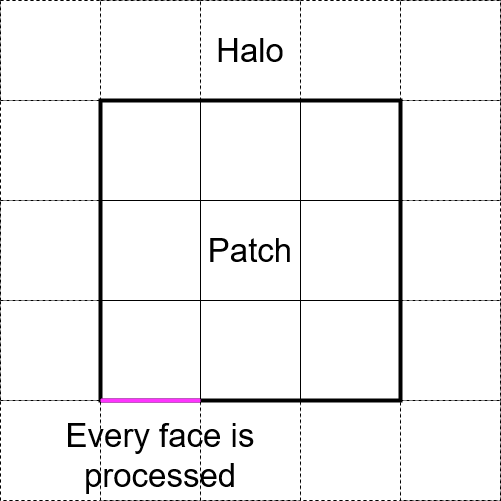
\includegraphics[width=.2\textwidth]{patch.png}
        \caption{Example of a 3x3 patch, with a halo of cells.}
        \label{fig:patch}
    \end{center}
\end{figure}


In summary, \proc{Patch Update} is a function whose input is: a haloed patch; a timestep; and patch meta-data such as its size in space. And whose output is: the patch (without a halo) that has been progressed in time. 

Calculating the flux and NCP at a shared face between 2 cells a non-trivial task.
This is because the face is at a discontinuity between the states of the 2 cells, and is known as the Riemann problem in FV.
As such, we require a scheme to solve the Riemann problem, which we will call the \proc{Numerical Ingredient}.
Many such schemes exist, such as Upwind and Downwind schemes, and the correct scheme to use depends on the problem.
Within ExaHyPE the Rusanov scheme \cite{rusanov} is used by default, as it well serves the role of a general \proc{Numerical Ingredient}.
The \proc{Numerical Ingredient} has an input of 2 cells and meta data about the face (e.g. its position in space).
And outputs 2 state vectors describing the change of state experienced by each cell.

At the bottom level of this hierarchy we have the \proc{Problem Descriptions}.
These are a collection of user defined functions the calculate: flux, NCP, source terms, and maximum eigenvalues.
All these functions share a similar input interface, taking single cell and the meta data for that cell.
And they output either a state vector or single value, depending on what quantity they are calculating.
In the default ExaHyPE setup, it will be \proc{Patch Update} that calls the source term function.
And \proc{Numerical Ingredient} that calls the flux, NCP and max eigenvalue functions.

A summary of the abstraction hierarchy of \proc{Patch Update} can be found in Table \ref{tab:patch_update}

\begin{table}
\begin{tabular}{lllcc}
    \toprule
    Process & User/Engine &Uses Functions & Input Size & Output Size\\
    \midrule
    \proc{Patch Update} (\proc{PU})&Engine& \makecell[l]{\proc{NI}, \proc{PD}\\ (source term)} & $q \cdot (p+2)^d+m$ & $q\cdot p^d$\\
    \proc{Numerical Ingredient} (\proc{NI}) &\makecell[l]{Engine \\(default),\\ User}& \makecell[l]{\proc{PD} (flux, ncp,\\ max eigenvalues)} & $2q+m$ & $2q$\\
    \proc{Problem Descriptions} (\proc{PD}) & User& - & $q+m$ & $q$ or $1$\\
    \bottomrule
\end{tabular}
\caption{A summary of the level of abstraction within the \proc{Patch Update} function. $p$ is the number of cells along 1 dimension in a patch, $d$ is the dimension of the patch, $q$ are the number of state variables, $m$ is the size of patch/state metadata.}\label{tab:patch_update}
\end{table}

Now we have an understanding of \proc{Patch Update} we can investigate some of the potential performance issues it experiences.
% ISSUE: lambda functions, not inline
Firstly, as mentioned at the beginning of this section, ExaHyPE implements the function pointer pattern to interface between user and engine code.
As such, the definition of \proc{Patch Update} looks like this:
\begin{lstlisting}[language=c]
void full_numerical_ingredient(
    std::function<...> flux, std::function<...> ncp,
    /* other args */);
void full_patch_update(
    std::function<...> numerical_ingredient, std::function<...> source_term,
    /* other args */);

void engine_core(){
    std::function<...> numerical_ingredient = [&](/*other args*/){
        full_numerical_ingredient(
            user_land::flux, user_land::ncp, /* other args*/
        );
    };
    std::function patch_update = [&](/*other args*/){
        full_patch_update(
            numerical_ingredient, user_land::source_term, /*other args */
        );
    };

    patch_update(double * in_patch, double * out_patch, ...);
}
\end{lstlisting}
This is non-trivial to fully inline, hence there is the potential the compiler choices to make function calls.
However, function calls hinder vectorization, therefore this code may not be vectorized well.


% ISSUE: heap allocation
The next issue we encounter is the use of heap allocation.
The implementation of \proc{Patch Update} allows us to use a single function for many different user codes.
However, this also means algorithmic precautions must be take to safely handel any user codes.
Within both \proc{Patch Update} and \proc{Numerical Ingredient} temporary variables are used to receive the result of function calls.
The size of these temporary variables depend on the size of a cells state.
Hence, safe behaviour dictates that these temporary variables are declared on the heap as opposed to the stack, which is slow. 


% ISSUE: branching
% MAYBE ISSUE: consts as function arguments



% ISSUE: repeated + unused comp
The final issue we will acknowledge is the existence of repeated and unused computations.
As we saw, every functional call within \proc{Patch Update} takes a meta data argument.
Some of this meta data needs to be calculated for every function call.
For example, \proc{Numerical Ingredient} requires the coordinates for the center of the face it is processing.
These coordinates are calculated using the coordinates of the 2 cells that share this face.
However, \proc{Numerical Ingredients} such as Rusanov use this coordinate.
Hence, we run the risk of the compiler not eliminating this redundant computation, especially as its definition and usage lie across different functions. 
Beyond unused computation, there can also be repeated computation.
If we look at using Rusanov as our \proc{Numerical Ingredient} there are many repeated computations.
To calculate the flux at the shared face of 2 cells $a,b$ Rusanov calculates $flux(a), flux(b), max\_eigenvalue(a), max\_eigenvalue(b)$.
The flux at the face is then a function of these 4 values.
If we were to then calculate the flux between $b,c$ note that the computation of $flux(b), max\_eigenvalue(b)$ is repeated.
It may be challenging for the compiler to spot this repetition, especially as it again lies across multiple different functions.
Furthermore, \proc{Patch Update} cannot be optimised to take advantage of this property of Runsnov, as it would no longer work with any \proc{Numerical Ingredient}.

To summarize, \proc{Patch Update} has the constraint of supporting any \proc{Numerical Ingredient} or \proc{Problem Description}. 
Within \proc{Patch Update} the function pointer patten and safe behaviour such as heap allocation is used to meet this constraint.
However, this constraint is in contension with performance.
Although optimisations can be made for specific pairings of \proc{Numerical Ingredient} and \proc{Problem Description}, there is limited scope for general optimisations. 
And at the end of the day, case by case optimisation detracts from the draw of using a PDE engine in the first place.

It is desirable to use a technique that maintains the modularity of \proc{Patch Update} but increases potential for optimisation.
This is what we will explore, applying a compiler based approach to achieve these goals.

